\documentclass[main.tex]{subfiles}
\begin{document}
\begin{bmcsexample}[Bond plasticity]
\noindent This example shows the response of bond material point 
with kinematic hardening with unloading and reloading.
 \\[3mm]
\begin{center}
            
{\scriptsize 
\begin{longtable}{lrp{4cm}}\toprule
\textbf{\textsf{Model parameter}} 
& 
\textbf{\textsf{Symbol = Value [Unit]}} 
&
\textbf{\textsf{Description}}  \\\midrule \midrule
\texttt{n\_steps} & $n_\mathrm{s}$ = 2000 [-] & {\footnotesize None}  \\
            \texttt{material\_model} & option = plasticity [-] & {\footnotesize None}  \\
            \texttt{interaction\_type} & option = predefined [-] & {\footnotesize None}  \\
            \midrule
\multicolumn{3}{l}{\textbf{\textsf{LoadingScenario: loading\_scenario}}}\\

\texttt{loading\_scenario.number\_of\_cycles} & $n_\mathrm{cycles}$ = 2 [-] & {\footnotesize None}  \\
            \texttt{loading\_scenario.number\_of\_increments} & $n_{\mathrm{incr}}$ = 20 [-] & {\footnotesize None}  \\
            \texttt{loading\_scenario.loading\_type} & option = cyclic [-] & {\footnotesize None}  \\
            \texttt{loading\_scenario.maximum\_loading} & $\phi_{\max}$ = 0.005 [-] & {\footnotesize None}  \\
            \texttt{loading\_scenario.amplitude\_type} & option = constant [-] & {\footnotesize None}  \\
            \texttt{loading\_scenario.unloading\_ratio} & $\phi_{\mathrm{unload}}$ = 0.5 [-] & {\footnotesize None}  \\
            \texttt{loading\_scenario.loading\_range} & option = non-symmetric [-] & {\footnotesize None}  \\
            
\multicolumn{3}{r}{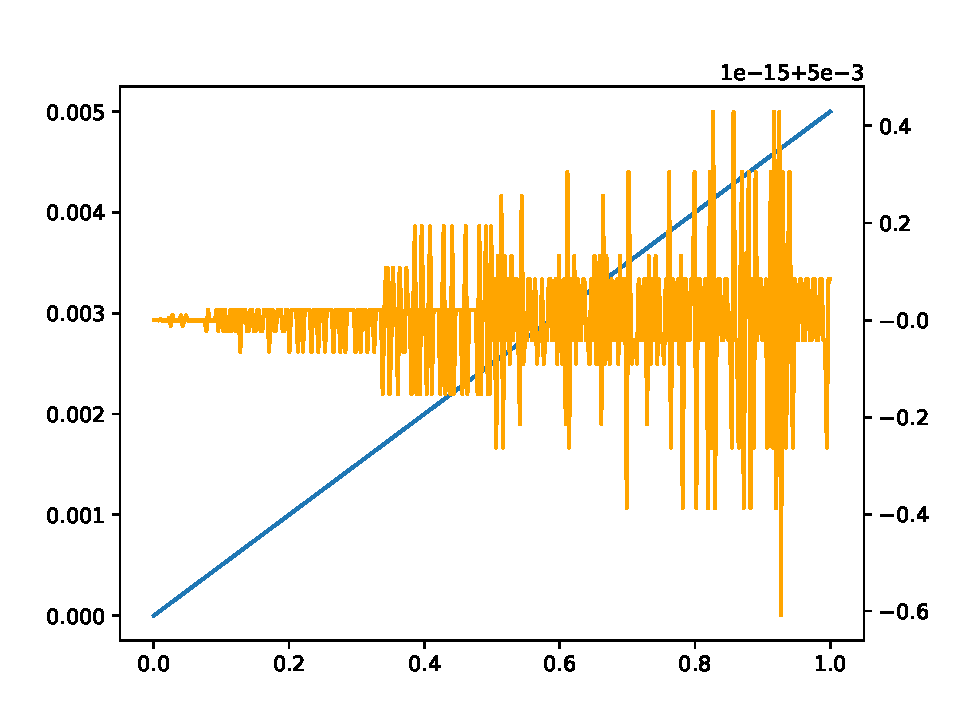
\includegraphics[width=5cm]{examples/e22_bond_slip_plasticity_kinem/fig_loading_scenario.pdf}}\\
\midrule
\multicolumn{3}{l}{\textbf{\textsf{MATSBondSlipEP: mats\_eval}}}\\

\texttt{mats\_eval.E\_b} & $E_\mathrm{b}$ = 12900 [MPa/mm] & {\footnotesize Bond stiffness}  \\
            \texttt{mats\_eval.K} & $K$ = 0.0 [MPa/mm] & {\footnotesize Isotropic hardening modulus}  \\
            \texttt{mats\_eval.tau\_bar} & $\bar{\tau}$ = 5 [MPa] & {\footnotesize Yield stress}  \\
            \texttt{mats\_eval.gamma} & $\gamma$ = 2000.0 [MPa/mm] & {\footnotesize Kinematic hardening modulus}  \\
            \bottomrule 
\end{longtable}
}

\noindent
\begin{tabular}{L{7.5cm}L{7.5cm}}
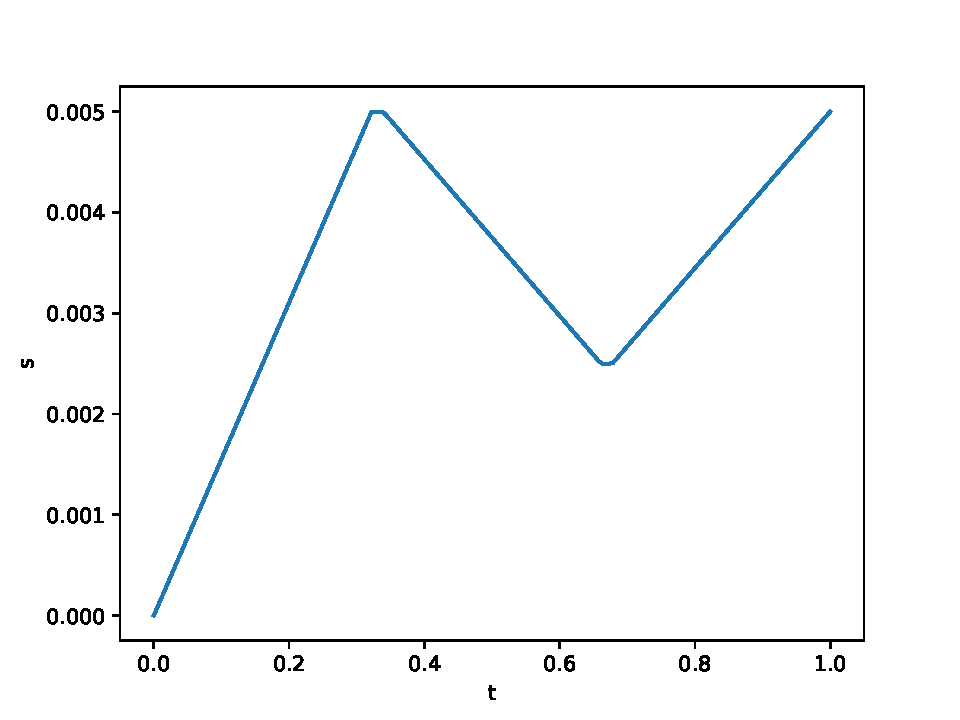
\includegraphics[width=7.5cm]{examples/e22_bond_slip_plasticity_kinem/fig_s-t.pdf}
 & 
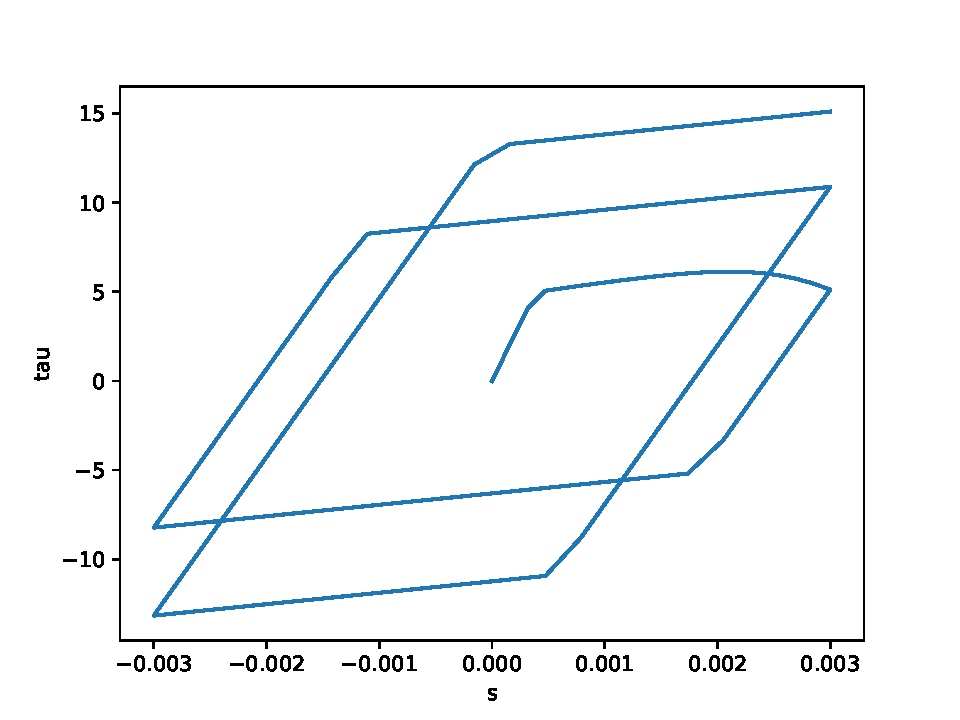
\includegraphics[width=7.5cm]{examples/e22_bond_slip_plasticity_kinem/fig_tau-s.pdf}
 \\\end{tabular}

\noindent
\begin{tabular}{L{7.5cm}L{7.5cm}}
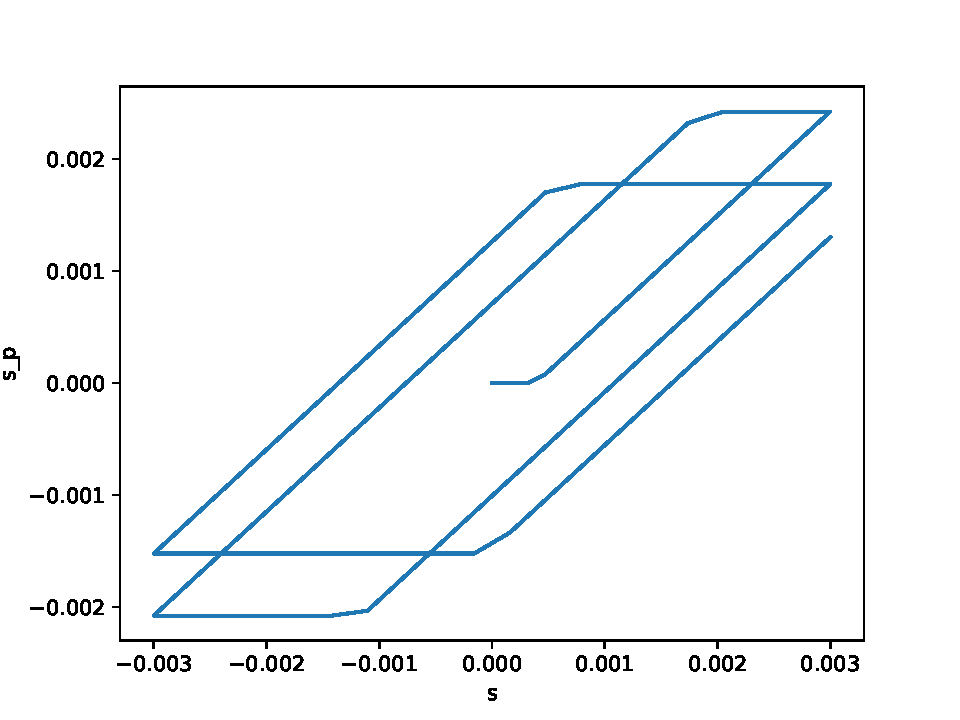
\includegraphics[width=7.5cm]{examples/e22_bond_slip_plasticity_kinem/fig_s_p-s.pdf}
 & 
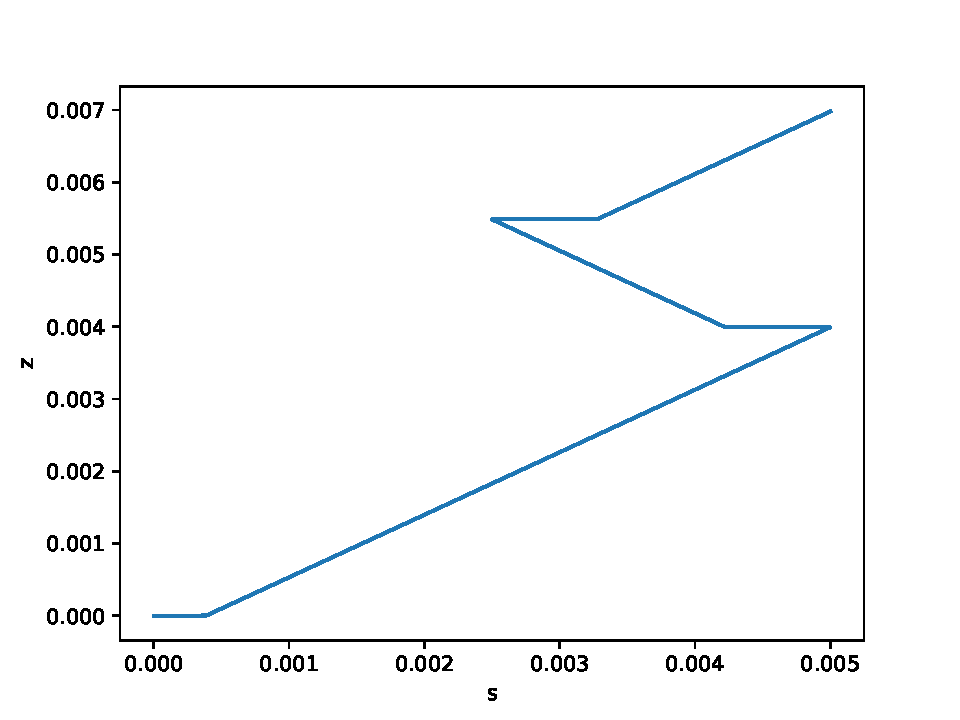
\includegraphics[width=7.5cm]{examples/e22_bond_slip_plasticity_kinem/fig_z-s.pdf}
 \\\end{tabular}
\end{center}
\end{bmcsexample}
\end{document}
    